\documentclass[a4paper]{ctexart}
\CTEXsetup[format={\Large\bfseries}]{section}
%\everymath{\displaystyle}
\usepackage{cleveref,float}
\usepackage{geometry,bm}
\usepackage{makecell,pifont}
\usepackage{multirow}
\usepackage{booktabs}
\usepackage{graphicx}
\geometry{
  left=17mm,
  right=17mm,
  top=17mm, 
  bottom=17mm,
}
\usepackage{subfigure}
\usepackage{hyperref}
\hypersetup{
    colorlinks=true,
    linkcolor=black,
    filecolor=black,      
    urlcolor=black,
    citecolor=black,
}
\usepackage{amsmath}
\usepackage{ntheorem}
\theorembodyfont{\songti}
\newtheorem{example}{\hskip 2em 例}[section]
\newtheorem*{zm}{\hskip 2em 证明}
\newtheorem*{sol}{\hskip 2em 解}
\usepackage{fancyhdr}
\fancypagestyle{plain}{
\fancyhf{}
\fancyhead[RE]{} % 在偶数页的右侧显示章名,
\fancyhead[LO]{} % 在奇数页的左侧显示小节名,
\fancyhead[LE,RO]{~\thepage~} % 在偶数页的左侧,奇数页的右侧显示页码
\fancyhead[CE]{近景摄影测量复习}		
\fancyhead[CO]{近景摄影测量复习}	
\renewcommand{\headrulewidth}{0.7pt}
\renewcommand{\footrulewidth}{0pt}
}
\title{近景摄影测量复习}
\author{SHZ}
\begin{document}
\maketitle
\thispagestyle{empty}
\clearpage
\begin{center}
\tableofcontents
\end{center}
\thispagestyle{empty}

\newpage
\setcounter{page}{1}
\pagestyle{plain}
\section{绪论}
1. 近景摄影测量的定义

通过摄影手段以确定(地形以外)目标的外形和运动状态的学科分支

2. 与航空摄影的比较
\begin{table}[h]
\centering
\begin{tabular}{cccc}
\toprule
\multicolumn{2}{c}{}         & 航空摄影                     & 近景摄影                          \\ 
\midrule
\multicolumn{2}{c}{相同点}      & \multicolumn{2}{l}{\makecell[c]{基本原理相同;模拟、解析、数字处理方法相同;\\某些内业摄影测量仪器的使用}} \\ 
\multirow{7}{*}{不同点} & 测量目的    & 地形、地貌,注重绝对位置             & 形状、大小、运动状态,不注重绝对位置            \\ 
                     & 目标物     & 地形、地貌                    & 千差万别                          \\ 
                     & 比例尺变化范围 & 不大                       & 较大                            \\ 
                     & 摄影方式    & 近似竖直                     & 正直、交向                         \\ 
                     & 影像获取设备  & 航摄仪                      & 量测摄影机、非量测摄影机                  \\ 
                     & 控制方式    & 控制点                      & 控制点、人工标志                      \\ 
                     &         &                          & 适合动态目标                        \\ 
\bottomrule
\end{tabular}
\end{table}

3. 近景摄影测量的优缺点

(1)优点:\ding{172}瞬间获取被测目标的大量几何和物理信息,适合于测量点数众多的目标;

\ding{173}非接触测量手段,可在恶劣条件下作业;

\ding{174}适合动态目标测量

\ding{175}适合微观目标测量。

(2)缺点:\ding{172}技术含量高,需较昂贵的设备和高素质人员;

\ding{173}对以下目标非最佳选择:不能获得质量合格的目标、待测量点数稀少。

4. 精度统计指标

主要是坐标中误差:\ding{172}估算精度;\ding{173}内精度;\ding{174}外精度。

5. 影像精度的因素

(1)像点坐标的质量

(2)摄影条件、摄影方式、控制质量

(3)图像处理与摄影测量处理的能力、水平

6. 近景摄影测量常用坐标系

(1)像平面坐标系:$(x,y)$

(2)像空间坐标系:$(x,y,-f)$

(3)像空间辅助坐标系:$(X_m,Y_m,Z_m)$

(4)物方空间坐标系:$(X,Y,Z)$
\section{近景摄影测量的影像获取设备}
1. 影像获取设备分类
$$
\begin{cases}
	\text{摄影设备}\begin{cases}
	\text{格网摄影机}\\
	\text{量测摄影机}\\
	\text{半量测摄影机}\\
	\text{非量测摄影机}\\
\end{cases}\\
	\text{摄像设备}\begin{cases}
	\text{工业相机}\\
	\text{数码相机}\\
	\text{电视摄像机}\\
	\text{高分辨率电视摄像机}\\
	\cdots \cdots\\
\end{cases}\\
\end{cases}
$$

2. 量测摄影机与非量测摄影机
\begin{table}[h]
\centering
\begin{tabular}{ccc}
\toprule
       & 非量测摄影机            & 量测摄影机          \\ 
\midrule
结构     & 不是专为测量目的而设计,结构不严谨 & 专为测量目的而设计,结构严谨 \\ 
内方位元素  & 未知且不能记录           & 已知、可记录         \\ 
外部定向设备 & 无                 & 有              \\ 
光学畸变差  & 大                 & 小              \\ 
改正底片变形 & 无                 & 采取措施压平底片       \\ 
其它     & 使用方便;普及、社会拥有量大    & 有机械或光学框标       \\ 
\bottomrule
\end{tabular}
\end{table}

3. 半量测摄影机与格网摄影机

(1)半量测摄影机:不具备量测摄影机的性能;具有改正底片变形的格网。(非量测摄影机加装格网)

(2)格网摄影机:具备量测摄影机的性能;还具有改正底片变形的格网。

5. 瑞士 Wild P31 型量测摄影机与德国 UMK 型量测摄影机

\begin{table}[h]
\centering
\begin{tabular}{ccc}
\toprule
     & 瑞士 Wild P31    & 德国 UMK    \\ 
\midrule
焦距   &\makecell[c]{45mm\quad P31/45\\100mm\quad P31/100\\200mm\quad P31/200}&\makecell[c]{65mm\quad UMK6.5/1318\\100mm\quad UMK10/1318\\200mm\quad UMK20/1318\\300mm\quad UMK/1318}           \\ 
结构   & \multicolumn{2}{c}{镜箱+支架} \\ 
像幅   & 102mm$\times$127mm&130mm$\times$180mm\\ 
有效面积&92mm$\times$118mm&120mm$\times$166mm\\ 
畸变差  &小于 $4\mu$m&小于 $12\mu$m\\ 
调焦   &更换垫圈改变主距&连续调焦改变主距\\ 
框标   &5 个,主点偏心&4 个\\ 
定向   &  \multicolumn{2}{c}{有外部定向设备}\\ 
胶卷   &使用干板或单张软片&使用干板或单张、成卷软片\\ 
格网   & \multicolumn{2}{c}{无}     \\ 
压平   &单张软片、干板压平措施不利&成卷软片可抽气压平\\
连续摄影 &不能&成卷软片可进行连续摄影\\ 
\bottomrule
\end{tabular}
\end{table}

6. 立体量测摄影机

立体量测摄影机所摄像对是正直摄影立体像对;可同步摄影,用于动态目标

7. 摄影机改变主距的方法

(1)连续调焦,改变主距,如 UMK 相机、普通相机

(2)更换垫圈,改变主距,如 P31 相机

(3)更换镜头,改变主距,如 CRC$-$1 相机、普通相机

8. 固态摄像机的分类

$$
\text{固态摄像机}\begin{cases}
	\text{按结构分}\begin{cases}
	\text{线阵相机}\\
	\text{面阵相机}\\
\end{cases}\\
	\text{按性能分}\begin{cases}
	\text{标准视频幅面摄像机}\\
	\text{高分辨率电视摄像机}\\
	\text{静止视频画面照相机}\\
\end{cases}\\
	\text{按分辨率分}\begin{cases}
	\text{低分辨率相机}\\
	\text{中分辨率相机}\\
	\text{高分辨率相机}\\
\end{cases}\\
\end{cases}
$$
\newpage
\section{近景摄影测量的摄影技术}
1. 正直摄影方式

摄影时,两摄影机主光轴相互平行且垂直于摄影基线的摄影方式。适合模拟、解析、数字近景摄影测量,影像具有一定的重叠度。

2. 交向摄影方式

摄影时,两摄影机主光轴大体位于同一平面内且不平行、不同时垂直于摄影基线的摄影方式。适合解析、数字近景摄影测量,常采用 100\% 重叠方式。

3. 正直摄影的精度估算式

\begin{table}[h]
\centering
\begin{tabular}{cc}
\toprule
符号 &意义  \\
\midrule
$(x_1,y_1)$,$(x_2,y_2)$ &$a_1$,$a_2$ 在各自像片坐标系中的坐标  \\
$H$ &摄影距离 $-Z$  \\
$B$ &摄影基线  \\
$f$ &摄影机主距  \\
$p$ &左右视差,$p=x_1-x_2$  \\
$m_p$ &左右视差中误差  \\
$m_x$ &$x$ 方向像点中误差 \\
$m_y$&$y$ 方向像点中误差\\
\bottomrule
\end{tabular}
\end{table}
(1)以 $(x,y,p)$ 为观测值

相当于立体观测时的量测情况,$\begin{cases}
	X=\frac{B}{p}\cdot x\\
	Y=\frac{B}{p}\cdot y\\
	Z=\frac{B}{p}\cdot f\\
\end{cases}$
$$
m_X=\pm \sqrt{k_{1}^{2}k_{2}^{2}\left( \frac{x}{f} \right) ^2m_{p}^{2}+k_{2}^{2}m_{x}^{2}}
$$
$$
m_Y=\pm \sqrt{k_{1}^{2}k_{2}^{2}\left( \frac{y}{f} \right) ^2m_{p}^{2}+k_{2}^{2}m_{y}^{2}}
$$
$$
m_Z=\pm k_1k_2m_p
$$
其中,$k_1=\frac{H}{B}$,$k_2=\frac{H}{f}$. 

得到的结论:

\ding{172}为提高精度,应尽可能拍摄摄影比例尺大的像片,即尽可能减小摄影距离,选用主距大的摄影机

\ding{173}为提高精度,应尽可能拍摄摄影基线大的像对

\ding{174}为提高精度,应尽可能提高像点坐标的质量,包括像点坐标的量测质量、剔除各类系统误差的能力

\ding{175}一般情况下,摄影方向的中误差最大,常以 $m_Z$ 估算精度

(2)以 $(x_1,y_1)$,$(x_2,y_2)$ 为观测值的估算式

$$
m_X=\pm m_x\cdot k_2\sqrt{2k_{1}^{2}\left( \frac{x}{f} \right) ^2+1}
$$
$$
m_Y=\pm \sqrt{2k_{1}^{2}k_{2}^{2}\left( \frac{y}{f} \right) ^2m_{x}^{2}+k_{2}^{2}m_{y}^{2}}
$$
$$
m_Z=\pm \sqrt{2}k_1k_2m_x
$$

4. 调焦距 $D$

在摄影方向上,摄影中心与调焦最清晰点间的距离。通俗的说即为摄影距离。

5. 超焦距 $H$

给定光圈和模糊圈的大小,当摄影机调焦到无穷远时,从摄影中心开始的某一距离到无穷远范围内的景物成像都是清晰的,这一距离称为超焦距。此清晰点称为无穷远起点。
$$
H=\frac{F^2}{k\cdot E}
$$
其中,$k$ 为光圈号数,$E$ 为模糊圈直径,$F$ 为摄影机焦距。从摄影角度看,超焦距以远的目标,其距离都认为是无穷远,构像均认为是清晰的。

6. 景深

给定光圈和模糊圈大小,在某一调焦距下,被摄影空间能够获得清晰构像的深度范围。景深 $\Delta D$ 为沿光轴方向的后景距 $D_2$ 与前景距 $D_1$ 的差值,$\Delta D=D_2-D_1$。

前景距 $D_1=\frac{H\cdot D}{H+D}$,后景距 $D_2=\frac{H\cdot D}{H-D}$,景深 $\Delta D=\frac{2H\cdot D^2}{H^2-D^2}$

7. 曝光时间的确定

已知用普通相机测光时,正确的曝光参数为:相机上安置的感光度为 $s$,光圈号数为 $k$,测得的曝光时间为 $t$(光圈优先)。近景摄影机使用的底片感光度为 $S$,安置光圈号数为 $K$,则应安置的正确曝光时间 $T$ 为:
$$
T=\frac{s}{S}\cdot \left( \frac{K}{k} \right) ^2\cdot t
$$
其中感光度单位采用 ISO 制。

\begin{example}
如用一架普通 135 相机对某目标进行测光,安置的感光度为 ISO100,光圈号数安置为 8,此时测得 的曝光时间为 1/60 秒。用 P31 摄影机对此目标摄影,选用的感光材料的感光度为 ISO400,安置的光圈号数为 11,试确定其正确的曝光时间。
\end{example}
\begin{sol}
$$
T=\frac{s}{S}\cdot \left( \frac{K}{k} \right) ^2\cdot t=\frac{100}{400}\cdot \left( \frac{11}{8} \right) ^2\cdot \frac{1}{60}\approx \frac{1}{127}
$$
\end{sol}

8. 光圈号数的确定(快门优先)

已知用普通相机测光时,正确的曝光参数为:相机上安置的感光度为 $s$,曝光时间为 $t$,测得的光圈号数为 $k$(时间优先);近景摄影机使用的底片感光度为 $S$,安置曝光时间为 $T$,则应安置的正确光圈号数 $K$ 为
$$
K=k\sqrt{\frac{S\cdot T}{s\cdot t}}
$$
其中感光度单位采用 ISO 制。

9. 静态目标立体像对的获取方法
$$
\begin{cases}
	\text{使用立体摄影机或立体摄影系统}\\
	\text{使用两台单个摄影机}\\
	\text{使用单个摄影机}\begin{cases}
	\text{移动相机法}\\
	\text{移动目标法}\\
	\text{旋转目标法}\\
	\text{投影标准格网法}\\
	\text{利用分光装置法}\\
\end{cases}\\
\end{cases}
$$

10. 动态目标立体像对获取方法
$$
\begin{cases}
	\text{同步快门}\begin{cases}
	\text{机械}\\
	\text{电子}\\
\end{cases}\\
	\text{计时装置}\\
	\text{频闪照明}\begin{cases}
	\text{主动}\\
	\text{被动}\\
\end{cases}\\
	\text{立体摄影的同一物镜法}\\
\end{cases}
$$

11. 被测物体的表面处理方法

目的:是为了提高影像的同名点识别能力,包括人工识别和自动识别。

(1)利用投影设备将光栅、格网、及图案、图像投影到物体表面,形成人工纹理;

(2)利用激光经纬仪、激光笔,按一定规则将激光投射到被测目标上,形成人工纹理;

(3)在被测目标表面粘贴人工标志,形成人工纹理;

(4)在被测目标表面上绘制人工纹理;

12. 照明的基本原则

(1)使用自然光、人工光源时,要照度均匀,避免出现反差过大的现象; 

(2)使用人工光源时照明灯要布置适宜;

(3)有些情况下要注意局部照明,如黑暗情况下的控制点、标准尺照明;

(4)特殊光源的使用。
\newpage
\section{近景摄影测量的控制}
1. 近景摄影测量控制的目的

(1)把所构建的近景摄影测量网纳入到给定的物方空间坐标系中;

(2)利用多余的控制(包括控制点和相对控制)加强近景摄影测量网的强度;

(3)利用多余的控制点和相对控制检查近景摄影测量的精度和可靠性。

2. 控制点

控制点通常是布设在被测目标上或其周围的已知坐标的标志点。

待定点坐标的中误差 $m$ 由控制点坐标中误差 $m_\text{控}$ 和摄影测量中误差 $m_\text{摄}$ 组成。
$$
m=\sqrt{m_{\text{控}}^{2}+m_{\text{摄}}^{2}}
$$
为使控制点坐标中误差 $m_\text{控}$ 对待定点坐标的中误差 $m$ 不产生影响,应使:$m_\text{控}<\frac{m_\text{摄}}{3}$

3. 相对控制

相对控制是指在近景摄影测量中布置在物方空间的未知点间的某种已知几何关系。

4. 控制点的一般测量方法:前方交会$+$三角高程

前方交会测量控制点的平面坐标;三角高程测量控制点的高程。

(1)平面精度分析
$$
M_P=\sqrt{\frac{m^2}{\rho ^2}\cdot \frac{a^2+b^2}{\sin ^2\gamma}+m_{A}^{2}\left( \frac{a}{S} \right) ^2+m_{B}^{2}\left( \frac{b}{S} \right) ^2}
$$
其中,$m_A$、$m_B$是测站点 $A$、$B$ 的点位中误差,$m$是内角 $A$、$B$ 的测角中误差,$S$是基线 $AB$ 的长度,$\gamma$ 是交会角。

(2)高程精度分析
$$
M_h=\sqrt{\tan ^2\alpha \cdot m_{D}^{2}+\left( \frac{D}{\cos ^2\alpha} \right) ^2\cdot \left( \frac{m_{\alpha}}{\rho} \right) ^2}
$$
其中,$m_D$ 为测站点与待定点间的水平距离中误差,$m_\alpha$ 为垂直角的测角中误差,$\alpha$ 为垂直角。

5. 测站点的确定

两个测站的情况下,确定两测站的坐标,只需确定基线长度

标准尺法:在测量基线的前方,水平放置一根高精度的标准尺,按前方交会方法测得尺上两点的坐标后,计算其长度,求出它与尺长真值的比值,改化基线长度。

\textbf{标准尺水平放置步骤:}

(1)根据实际情况安置两测站 $A$、$B$ 后,近似量取基线长度 $S^{\prime}_{AB}$ 作为初值;

(2)在测量基线的前方,水平放置一根高精度的标准尺,在其上选取两个刻划 $M$、$N$,做出标记,其真长记为 $S_{MN}$;

(3)确定起始方向线;

(4)在两测站 $A$、$B$ 使用经纬仪,按前方交会法分别观测 $M$、$N$ 两点的水平角;

(5)按前方交会公式计算 $M$、$N$ 两点的平面坐标;

(6)计算 $M$、$N$ 两点间的距离 $S_{MN}=\sqrt{\left( X_M-X_N \right) ^2+\left( Y_M-Y_N \right) ^2}$;

(7)计算比例归划系数 $\lambda =\frac{S_{MN}}{S_{MN}^{'}}$

(8)求解测量基线长度 $S_{AB}=\lambda \cdot S_{AB}^{'}$

\textbf{标准尺任意放置步骤:}

(1)根据实际情况安置两测站 $A$、$B$ 后,近似量取基线长度 $S^{\prime}_{AB}$ 作为初值;

(2)在测量基线的前方,任意放置一根高精度的标准尺,在其上选取两个刻划 $M$、$N$,做出标记,其真长记为 $S_{MN}$;

(3)确定起始方向线;

(4)在两测站 $A$、$B$ 使用经纬仪,按前方交会法分别观测 $M$、$N$ 两点的水平角,按三角高程法分别观测 $M$、$N$ 两点的垂直角;

(5)按前方交会公式计算 $M$、$N$ 两点的平面坐标,按三角高程法分别计算 $M$、$N$ 两点的高程;

(6)计算 $M$、$N$ 两点间的距离 $S_{MN}=\sqrt{\left( X_M-X_N \right) ^2+\left( Y_M-Y_N \right) ^2+(Z_M-Z_N)^2}$;

(7)计算比例归划系数 $\lambda =\frac{S_{MN}}{S_{MN}^{'}}$

(8)求解测量基线长度 $S_{AB}=\lambda \cdot S_{AB}^{'}$

5. 起始方向线的确定方法

(1)内标志法

(2)对称目标法

(3)外标志法

(4)旋转仪器法

(5)外部定向点法

(6)平行光管法

6. 控制场建立的目的

(1)用于摄影机检定

(2)用于近景摄影测量理论的研究

(3)用于实测目标形状或运动状态

7. 控制点的布设原则

(1)布设足够数量的三维控制点标志,大小适宜;

(2)控制点应分布均匀,在空间上有足够延伸;

(3)留有摄影空间;

(4)建议制作带强制对中的观测墩。

8. 活动控制系统

均匀分布有一定数量已知坐标的控制点的可携带框架,称为活动控制系统。

9. 建立活动控制系统的目的

(1)被测目标较小,数量较多且处在不同的位置;

(2)不宜采用常规测量方法在现场实施控制测量;

(3)用于长途运输后摄影机的检校。
\newpage
\section{基于共线条件方程的近景像片处理方法}
1. 共线条件方程可以解算的结果

(1)可解算内方位元素 $(x_0,y_0,f)$

(2)可解算外方位元素 $(X_S,Y_S,Z_S,\varphi ,\omega,\kappa)$

(3)可解算物方空间坐标 $(X,Y,Z)$

(4)可解算系统误差参数,如畸变系数

(5)可解算像点坐标 $(x,y)$

2. 共线条件方程像点误差方程一般式
\begin{align*}
\left[ \begin{array}{c}
	v_x\\
	v_y\\
\end{array} \right] =&\left[ \begin{matrix}
	\frac{\partial x}{\partial X_S}&		\frac{\partial x}{\partial Y_S}&		\frac{\partial x}{\partial Z_S}&		\frac{\partial x}{\partial \varphi}&		\frac{\partial x}{\partial \omega}&		\frac{\partial x}{\partial \kappa}\\
	\frac{\partial y}{\partial X_S}&		\frac{\partial y}{\partial Y_S}&		\frac{\partial y}{\partial Z_S}&		\frac{\partial y}{\partial \varphi}&		\frac{\partial y}{\partial \omega}&		\frac{\partial y}{\partial \kappa}\\
\end{matrix} \right] \left[ \begin{array}{c}
	\Delta X_S\\
	\Delta Y_S\\
	\Delta Z_S\\
	\Delta \varphi\\
	\Delta \omega\\
	\Delta \kappa\\
\end{array} \right] +\left[ \begin{matrix}
	\frac{\partial x}{\partial X}&		\frac{\partial x}{\partial Y}&		\frac{\partial x}{\partial Z}\\
	\frac{\partial y}{\partial X}&		\frac{\partial y}{\partial Y}&		\frac{\partial y}{\partial Z}\\
\end{matrix} \right] \left[ \begin{array}{c}
	\Delta X\\
	\Delta Y\\
	\Delta Z\\
\end{array} \right] \\
&+\left[ \begin{matrix}
	\frac{\partial x}{\partial f}&		\frac{\partial x}{\partial x_0}&		\frac{\partial x}{\partial y_0}\\
	\frac{\partial y}{\partial f}&		\frac{\partial y}{\partial x_0}&		\frac{\partial y}{\partial y_0}\\
\end{matrix} \right] \left[ \begin{array}{c}
	\Delta f\\
	\Delta x_0\\
	\Delta y_0\\
\end{array} \right] -\left[ \begin{array}{c}
	x-\left( x \right)\\
	y-\left( y \right)\\
\end{array} \right] 
\end{align*}
也即 $\boldsymbol{V}=\boldsymbol{At}+\boldsymbol{BX}_1+\boldsymbol{CX}_2-\boldsymbol{L}$,如考虑各类系统误差改正,则误差方程一般式为 $\boldsymbol{V}=\boldsymbol{At}+\boldsymbol{BX}_1+\boldsymbol{CX}_2+\boldsymbol{DX}_{ad}-\boldsymbol{L}$其中 $\bm{D}$、$\bm{X}_{ad}$ 与选择的数学模型有关。如考虑将物方点分为控制点和待定点,则误差方程一般式为 $\boldsymbol{V}=\boldsymbol{At}+\boldsymbol{B}_c\boldsymbol{X}_c+\boldsymbol{B}_u\boldsymbol{X}_u+\boldsymbol{CX}_2+\boldsymbol{DX}_{ad}-\boldsymbol{L}$,此时,$\bm{D}$ 相应于具体的数学模型,$\bm{L}$ 中的 $(x)$、$(y)$ 应为
$$
\begin{cases}
	\left( x \right) =-f\frac{\overline{X}}{\overline{Z}}+x_0-\Delta x\\
	\left( y \right) =-f\frac{\overline{Y}}{\overline{Z}}+y_0-\Delta y\\
\end{cases}
$$

3. 多片空间前方交会

根据已知内、外方位元素的两张或两张以上的像片,将待定点的像点坐标视作观测值,按共线条件方程逐点解算待定点物方空间坐标的过程。
\begin{figure}[htbp]
\centering

\subfigure{
\begin{minipage}[t]{0.5\linewidth}
\centering
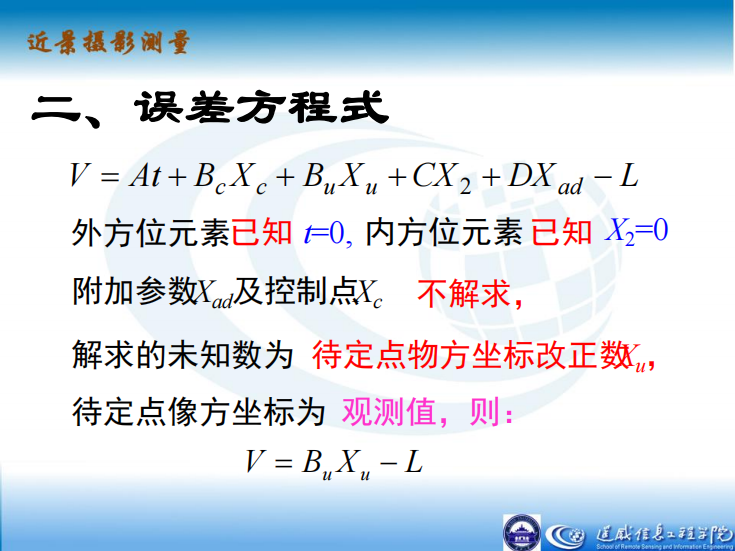
\includegraphics[scale=0.3]{img1.png}
%\caption{fig1}
\end{minipage}%
}%
\subfigure{
\begin{minipage}[t]{0.5\linewidth}
\centering
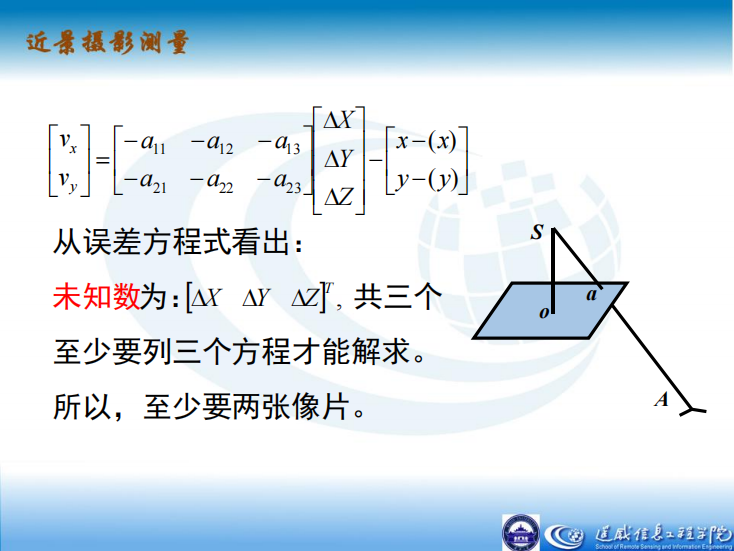
\includegraphics[scale=0.3]{img2.png}
%\caption{fig2}
\end{minipage}%
}%
\centering
\end{figure}

影响精度的因素:\ding{172}网的几何构形,包括像片张数、布局、交会角;

\ding{173}像点坐标的质量;

\ding{174}各像片外方位元素的测定精度;

\ding{175}摄影机内方位元素的检定水平。
\newpage
4. 单像空间后方交会

根据一张像片覆盖的一定数量控制点的物方 空间坐标及其像点坐标,以像点坐标作为观测值, 按共线条件方程解算该像片的内、外方位元素以 及其它附加参数的过程。

\begin{figure}[htbp]
\centering

\subfigure{
\begin{minipage}[t]{0.5\linewidth}
\centering
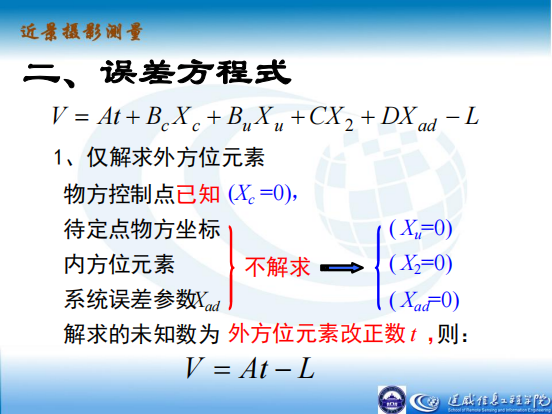
\includegraphics[scale=0.4]{img3.png}
%\caption{fig1}
\end{minipage}%
}%
\subfigure{
\begin{minipage}[t]{0.5\linewidth}
\centering
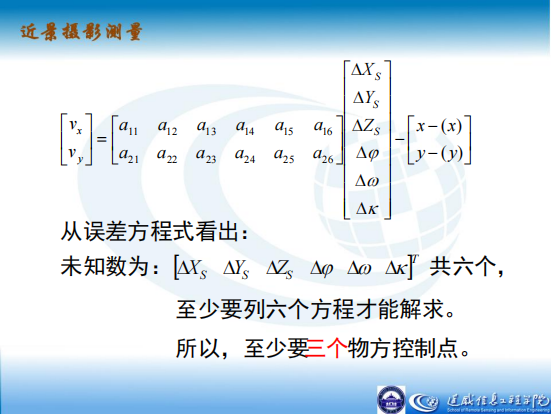
\includegraphics[scale=0.4]{img4.png}
%\caption{fig2}
\end{minipage}%
}%

\subfigure{
\begin{minipage}[t]{0.5\linewidth}
\centering
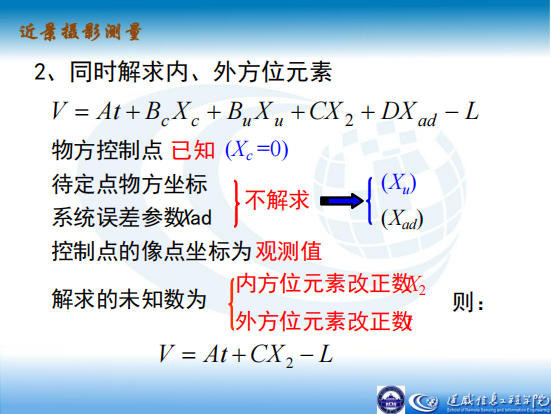
\includegraphics[scale=0.4]{img5.png}
%\caption{fig1}
\end{minipage}%
}%
\subfigure{
\begin{minipage}[t]{0.5\linewidth}
\centering
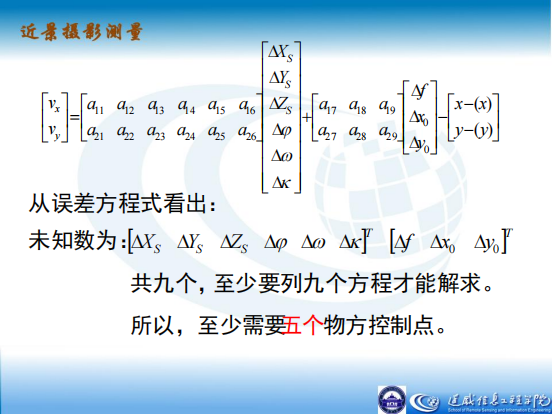
\includegraphics[scale=0.4]{img6.png}
%\caption{fig2}
\end{minipage}%
}%

\subfigure{
\begin{minipage}[t]{0.5\linewidth}
\centering
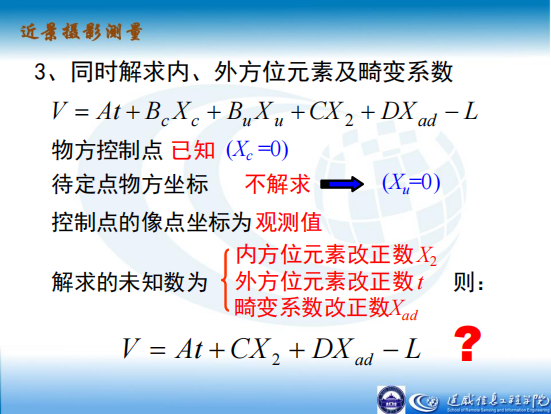
\includegraphics[scale=0.4]{img7.png}
%\caption{fig1}
\end{minipage}%
}%
\end{figure}

5. 光线束解法

(1)把控制点的像点坐标、待定点的像点坐标以 至其它内外业量测数据的一部分或全部均视作观 测值,按共线条件方程整体地、同时地解算它们的最或是值和待定点的物方空间坐标的解算方法。

(2)与空间后交—前交的区别:\ding{172}空间后方交会-空间前方交会解法分步解求,光线束法为整体解算;\ding{173}空间后交—前交解法中待定点的像点坐标对外方位元素的确定不起作用;光线束法中,待定点的像点坐标对外方位元素的确定有很大影响。

6. 几种典型的光线束解法

(1)控制点坐标视作真值且实地不测外方位元素的光线束解法

\ding{172} 适用条件

(a) 在被测目标上或周围可以布设稳固的控制点,分布合理,控制点精度好;

(b)使用量测摄影机,同一调焦距,或使用检校过的非量测相机,同一调焦距;

\ding{173}误差方程式
$$
\boldsymbol{V}=\boldsymbol{At}+\boldsymbol{B}_c\boldsymbol{X}_c+\boldsymbol{B}_u\boldsymbol{X}_u+\boldsymbol{CX}_2+\boldsymbol{DX}_{ad}-\boldsymbol{L}
$$

原则:对观测值列误差方程式

观测值:$\text{像点坐标}\begin{cases}
	\text{待定点像点坐标}\\
	\text{控制点像点坐标}\\
\end{cases}$

未知数:$\begin{cases}
	\text{待定点的物方空间坐标改正数}\\
	\text{外方位元素改正数}\\
\end{cases}$
$$
\begin{cases}
	\boldsymbol{V}_c=\boldsymbol{A}_c\boldsymbol{t}-\boldsymbol{L}_c\,\,, \boldsymbol{P}_c\\
	\boldsymbol{V}_u=\boldsymbol{A}_u\boldsymbol{t}+\boldsymbol{B}_u\boldsymbol{X}_u-\boldsymbol{L}_u\,\,, \boldsymbol{P}_u\\
\end{cases}
$$

(2)控制点坐标视作真值且实地不测外方位元素的光线束解法 

\ding{172}适用条件

(a)在被测目标上或周围可以布设稳固的控制点,分布合理,控制点精度好;

(b)使用未检校的非量测摄影机,同一调焦距
$$
\begin{cases}
	\boldsymbol{V}_c=\boldsymbol{A}_c\boldsymbol{t}+\boldsymbol{C}_c\boldsymbol{X}_2+\boldsymbol{D}_c\boldsymbol{X}_{ad}-\boldsymbol{L}_c\,\,, \boldsymbol{P}_c\\
	\boldsymbol{V}_u=\boldsymbol{A}_u\boldsymbol{t}+\boldsymbol{B}_u\boldsymbol{X}_u+\boldsymbol{C}_u\boldsymbol{X}_2+\boldsymbol{D}_u\boldsymbol{X}_{ad}-\boldsymbol{L}_u\,\,, \boldsymbol{P}_u\\
\end{cases}
$$

(3)无控制点且外方位元素视作观测值的光线束解法

\ding{172}适用条件

(a)在被测目标上或周围无法或不易布设控制点;

(b)使用量测摄影机,同一调焦距,或使用检校过的非量测相机,同一调焦距;

(c)实地可量测外方位元素,但精度不高,将其认做观测值。

\ding{173}误差方程式
$$
\boldsymbol{V}=\boldsymbol{At}+\boldsymbol{B}_c\boldsymbol{X}_c+\boldsymbol{B}_u\boldsymbol{X}_u+\boldsymbol{CX}_2+\boldsymbol{DX}_{ad}-\boldsymbol{L}
$$

原则:对观测值列误差方程式

观测值:$\begin{cases}
	\text{待定点像点坐标}\\
	\text{外方位元素}\\
\end{cases}$

未知数:$\begin{cases}
	\text{待定点的物方空间坐标改正数}\\
	\text{外方位元素改正数}\\
\end{cases}$
$$
\begin{cases}
	\boldsymbol{V}_u=\boldsymbol{A}_u\boldsymbol{t}+\boldsymbol{B}_u\boldsymbol{X}_u-\boldsymbol{L}_u\,\,, \boldsymbol{P}_u\\
	\boldsymbol{V}_E=\boldsymbol{t}\,\,, \boldsymbol{P}_E\\
\end{cases}
$$

(4)无控制点且外方位元素视作观测值的光线束解法

\ding{172}适用条件

(a)在被测目标上或周围无法或不易布设控制点;

(b)使用非量测摄影机,同一调焦距;

(c)实地可量测外方位元素,但精度不高,将其认做观测值。

\ding{173}误差方程式
$$
\boldsymbol{V}=\boldsymbol{At}+\boldsymbol{B}_c\boldsymbol{X}_c+\boldsymbol{B}_u\boldsymbol{X}_u+\boldsymbol{CX}_2+\boldsymbol{DX}_{ad}-\boldsymbol{L}
$$

原则:对观测值列误差方程式

观测值:$\begin{cases}
	\text{待定点像点坐标}\\
	\text{外方位元素}\\
\end{cases}$

未知数:$\begin{cases}
	\text{待定点的物方空间坐标改正数}\\
	\text{外方位元素改正数}\\
\text{内方位元素改正数}\\
\text{畸变系数改正数}
\end{cases}$
$$
\begin{cases}
	\boldsymbol{V}_u=\boldsymbol{A}_u\boldsymbol{t}+\boldsymbol{B}_u\boldsymbol{X}_u+\boldsymbol{C}_u\boldsymbol{X}_2+\boldsymbol{D}_u\boldsymbol{X}_{ad}-\boldsymbol{L}_u\,\,, \boldsymbol{P}_u\\
	\boldsymbol{V}_E=\boldsymbol{t}\,\,, \boldsymbol{P}_E\\
\end{cases}
$$

(5)控制点物方坐标及外方位元素均视作观测值的光线束解法

\ding{172}适用条件

(a)在被测目标上或周围布设有控制点,但看作观测值;

(b)使用量测摄影机,同一调焦距,或使用检校过的非量测相机,同一调焦距;

(c)实地可量测外方位元素,但精度不高。

\ding{173}误差方程式
$$
\boldsymbol{V}=\boldsymbol{At}+\boldsymbol{B}_c\boldsymbol{X}_c+\boldsymbol{B}_u\boldsymbol{X}_u+\boldsymbol{CX}_2+\boldsymbol{DX}_{ad}-\boldsymbol{L}
$$

原则:对观测值列误差方程式

观测值:$\begin{cases}
	\text{待定点像点坐标}\\
	\text{控制点像点坐标}\\
	\text{控制点物方坐标}\\
	\text{外方位元素}\\
\end{cases}$

未知数:$\begin{cases}
	\text{待定点的物方空间坐标改正数}\\
	\text{控制点的物方空间坐标改正数}\\
	\text{外方位元素改正数}\\
\end{cases}$
$$
\begin{cases}
	\boldsymbol{V}_u=\boldsymbol{A}_u\boldsymbol{t}+\boldsymbol{B}_u\boldsymbol{X}_u-\boldsymbol{L}_u\,\,, \boldsymbol{P}_u\\
	\boldsymbol{V}_c=\boldsymbol{A}_c\boldsymbol{t}+\boldsymbol{B}_c\boldsymbol{X}_c-\boldsymbol{L}_c\,\,, \boldsymbol{P}_c\\
	\boldsymbol{V}_{Sc}=\boldsymbol{X}_c\,\,, \boldsymbol{P}_{Sc}\\
	\boldsymbol{V}_E=\boldsymbol{t}\,\,, \boldsymbol{P}_E\\
\end{cases}
$$

(6)控制点物方坐标及外方位元素均视作观测值的光线束解法

\ding{172}适用条件

(a)在被测目标上或周围无法或不易布设控制点;

(b)使用非量测摄影机,同一调焦距;

(c)实地可量测外方位元素,但精度不高,将其认做观测值。

\ding{173}误差方程式
$$
\boldsymbol{V}=\boldsymbol{At}+\boldsymbol{B}_c\boldsymbol{X}_c+\boldsymbol{B}_u\boldsymbol{X}_u+\boldsymbol{CX}_2+\boldsymbol{DX}_{ad}-\boldsymbol{L}
$$

原则:对观测值列误差方程式

观测值:$\begin{cases}
	\text{待定点像点坐标}\\
	\text{控制点像点坐标}\\
	\text{控制点物方坐标}\\
	\text{外方位元素}\\
\end{cases}$

未知数:$\begin{cases}	
	\text{待定点的物方空间坐标改正数}\\
	\text{控制点的物方空间坐标改正数}\\
	\text{外方位元素改正数}\\
	\text{内方位元素改正数}\\
	\text{畸变系数改正数}\\
\end{cases}$
$$
\begin{cases}
	\boldsymbol{V}_u=\boldsymbol{A}_u\boldsymbol{t}+\boldsymbol{B}_u\boldsymbol{X}_u+\boldsymbol{C}_u\boldsymbol{X}_2+\boldsymbol{D}_u\boldsymbol{X}_{ad}-\boldsymbol{L}_u\,\,,\boldsymbol{P}_u\\
	\boldsymbol{V}_c=\boldsymbol{A}_c\boldsymbol{t}+\boldsymbol{B}_c\boldsymbol{X}_c+\boldsymbol{C}_c\boldsymbol{X}_2+\boldsymbol{D}_c\boldsymbol{X}_{ad}-\boldsymbol{L}_c\,\,,\boldsymbol{P}_c\\
	\boldsymbol{V}_{Sc}=\boldsymbol{X}_c+\boldsymbol{C}_{Sc}\boldsymbol{X}_2+\boldsymbol{D}_c\boldsymbol{X}_{ad}\,\,,\boldsymbol{P}_{Sc}\\
	\boldsymbol{V}_E=\boldsymbol{t}\,\,,\boldsymbol{P}_E\\
\end{cases}
$$
\newpage
\section{直接线性变换}
1. 定义

直接线性变换解法是建立像点的“坐标仪坐标”和相应物点的物方空间坐标直接的线性关系的解法。

2. 直接线性变换解法的特点

(1)不归心、不定向

(2)不需要方位元素的起始值

(3)物方空间需布置一组控制点

(4)特别适合于处理非量测相机所摄影像

(5)本质是一种空间后交-前交解法

3. 直接线性变换基本关系式
$$
\begin{cases}
	x+\frac{l_1X+l_2Y+l_3Z+l_4}{l_9X+l_{10}Y+l_{11}Z+1}=0\\
	y+\frac{l_5X+l_6Y+l_7Z+l_8}{l_9X+l_{10}Y+l_{11}Z+1}=0\\
\end{cases}
$$

由物方空间控制点及对应的像点解算 $l_i$ 系数的个数:11个

物方空间至少布置 6 个控制点 解算 $l_i$ 系数的近似值,不需平差计算只需选取11个方程解算11个 $l_i$ 未知数即,从控制点中挑出 5.5 个控制点列 11 个方程解算,或用所有控制点列线性方程组,解超定方程组。

3. 控制点空间分布的要求

控制点在空间分布均匀;在像片上的构像范围大。

4. 操作特点

(1)像片可任意放置,不归心、不定向;

(2) 既可单片量测像点坐标,也可立体量测像点坐标;

(3)对数字影像,在图像坐标系中量测控制点和待定点的影像坐标。量测精度有像素级和子像素级

5. 摄站位置安置的要求

摄站点不能与物方坐标系原点重合

6. 影响精度的因素

(1)像点坐标量测精度;

(2)控制点的数量、质量、分布;

(3)两像片主光轴的交会角

(4)像片张数

(5)非线性畸变误差的改正程度。
\end{document}